%(BEGIN_QUESTION)
% Copyright 2006, Tony R. Kuphaldt, released under the Creative Commons Attribution License (v 1.0)
% This means you may do almost anything with this work of mine, so long as you give me proper credit

Hvis vi lager et hull i bunnen av en beholder med en ellers statisk væskesøyle, kan vi bruke Bernoullis ligning i tre ulike punkter i systemet:

$$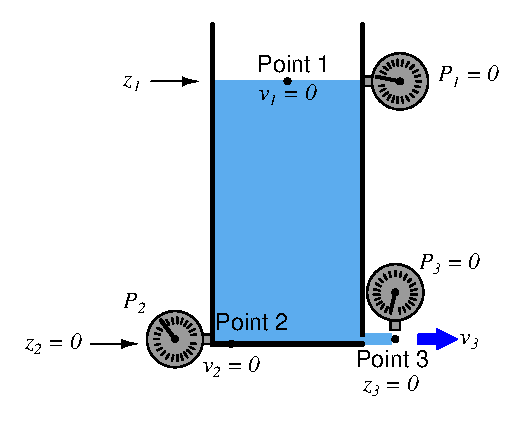
\includegraphics[width=15.5cm]{i00446x01.eps}$$

Merk at punkt 1 ikke har hastighet eller trykk, men har høyde; punkt 2 har ikke hastighet eller høyde, men har trykk; og punkt 3 har verken høyde eller trykk, men har hastighet.

Bruk Bernoullis ligning til å sette opp en ny ligning som knytter høyden i punkt 1 til trykket i punkt 2 og hastigheten i punkt 3. Løs deretter for hastigheten i punkt 3 uttrykt ved de andre to punktenes ikke-null variabler.

\vskip 10pt

\noindent
{\bf Bernoullis ligning:}

$$z_1 \rho g + {v_1^2 \rho \over 2} + P_1 = z_2 \rho g + {v_2^2 \rho \over 2} + P_2$$

\underbar{file i00446}
%(END_QUESTION)





%(BEGIN_ANSWER)

$$z_1 \rho g + {v_1^2 \rho \over 2} + P_1 = z_2 \rho g + {v_2^2 \rho \over 2} + P_2 = z_3 \rho g + {v_3^2 \rho \over 2} + P_3$$

$$z_1 \rho g + 0 + 0 = 0 + 0 + P_2 = 0 + {v_3^2 \rho \over 2} + 0$$

$$z_1 \rho g = P_2 = {v_3^2 \rho \over 2}$$

\vskip 10pt

$$v_3 = \sqrt{2 g z_1}$$

$$v_3 = \sqrt{2 P_2 \over \rho}$$

\vskip 10pt

Pitot-røret konverterer strømmens hastighetshode ($v^2 \rho \over 2$) til stagnasjonstrykk ($P$), og deretter til høydehode ($z \rho g$).

\vskip 10pt

Utfordringsspørsmål: forklar hvorfor et {\it Pitot-rør} plassert i utløpsstrømmen genererer en væskesøyle med samme høyde som $z_1$:

$$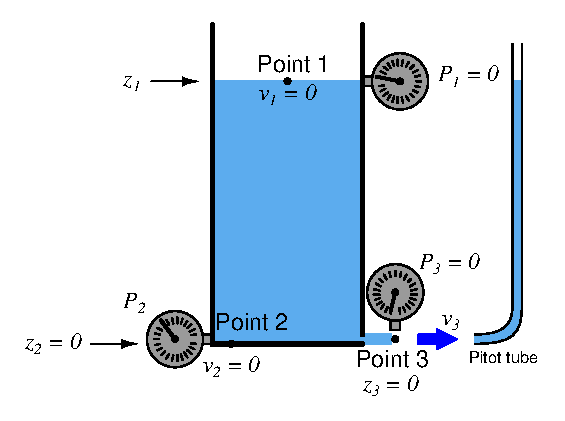
\includegraphics[width=15.5cm]{i00446x02.eps}$$

%(END_ANSWER)





%(BEGIN_NOTES)


%INDEX% Physics, dynamic fluids: Torricelli's theorem derived from Bernoulli's equation

%(END_NOTES)
